\documentclass[11pt]{article}
\usepackage[letterpaper,margin=1in]{geometry}
\usepackage{color}
\usepackage[dvipdfmx]{graphicx}
\usepackage{amsbsy}
\usepackage{amsmath}
\usepackage{adjustbox}
\usepackage{url}

\newcommand{\argmax}{\mathop{\rm arg~max}\limits}

\begin{document}
\title{Analysis Report on Assignment 6: Feature Engineering}
\author{Yoshinari Fujinuma}
\date{}
\maketitle

\section{Feature Engineering on the L2 regularized Logistic Regression}
Held out dev dataset.

Out of the 14,000 training examples, the first 10,000 examples are used during the training, the rest of 4,000 examples are used as the held out development dataset.

Features:

unigram

word embeddings

bigram

trope Names

Named entity 

Genre of the movie


After including enough features and throwing away the unigram feature, the accuracy of the prediction increased.

In the initial trial and errors, and looking into Jorndan's paper, some unigrmas such as ``kill'', ``death'' so even after we drop unigram features, we add them back to the mdoel.



\section{Error Analysis}
%The following two graph shows the relationship between training examples and accuracy:
%\begin{figure}[htb]
%  \begin{center}
%   \begin{tabular}{c}
%
%    \begin{minipage}{0.5\hsize}
%     \begin{center}
%     \scalebox{0.33}
%      {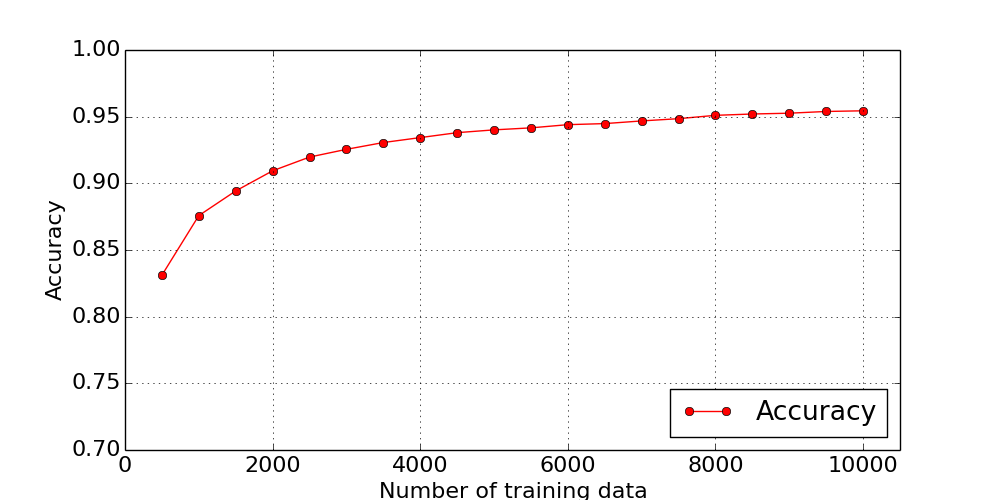
\includegraphics[]{figure_1.png}}
%   
%      \caption{The relationship between the number of training examples and accuracy. The value of $k$ is fixed to $3$. }
%      \label{fig:corpus_size}
%     \end{center}
%    \end{minipage}
%
%    \begin{minipage}{0.01\hsize}
%    \end{minipage}
%
%    \begin{minipage}{0.5\hsize}
%     \begin{center}
%      \scalebox{0.33}
%      {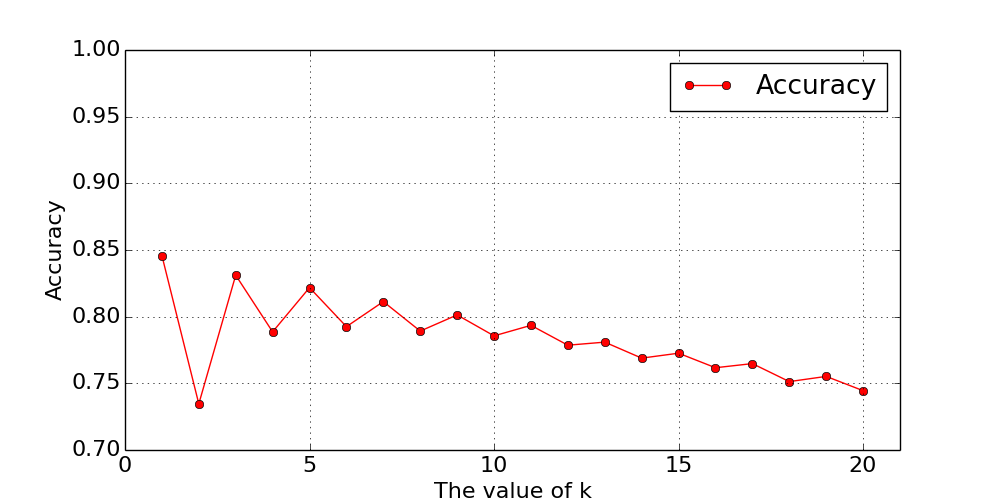
\includegraphics[]{figure_2.png}}
%      \caption{\label{k_and_accuracy}The relationship between $k$ and accuracy. The value of the number of training examples is fixed to $500$}
%     \end{center}
%    \end{minipage}
%
%  \end{tabular}
% \end{center}
%\end{figure}

\section{What numbers get confused with each other most easily?}

\end{document}

